\section{Tecniche utilizzate per le tracce delle matrici gamma}
Il calcolo del prodotto di spinori $(C)$ utilizzando la rappresentazione esplicita è già abbastanza lungo e noioso. Lo scattering Coulombiano infatti è un caso semplice (anche se non si direbbe). Infatti è stato sufficiente calcolare il modulo dell'elemento temporale
$$
\overline{u}_f \gamma^0 u_i = u_f^\dagger u_i
$$
dato che solo $A_0$ era diverso da zero. C'è una sola particella perchè calcoliamo uno scattering da potenziale (in casi più complessi abbiamo bisogno di tecniche più potenti). Introduciamo quindi queste tecniche partendo dal caso semplice dello scattering coulombiano. Prima di fare la semplificazione per un campo coulombiano statico abbiamo
$$
V_{fi} \sim \overline{u}_f \gamma^\mu u_i A_\mu
$$
Calcoliamo il modulo quadrato 
$$
|V_{fi}|^2 \sim (\overline{u}_f \gamma^\mu u_i A_\mu) (\overline{u}_f \gamma^\nu u_i A_\nu)^* = (\overline{u}_f \gamma^\mu u_i) (\overline{u}_f \gamma^\nu u_i)^* A_\mu A_\nu^*
$$
Consideriamo per il momento il caso di fascio non polarizzato senza misura della polarizzazione nello stato finale dobbiamo calcolare
$$
\overline{|V_{fi}|^2} = \sum_{if} |V_{fi}|^2 \qquad L^{\mu\nu} = \frac{1}{2} \sum_{i,f} (\overline{u}_f \gamma^\mu u_i) (\overline{u}_f \gamma^\nu u_i)^* \qquad \overline{|V_{fi}|^2} \sim L^{\mu\nu} A_\mu A_\nu^*
$$
Consideriamo il tensore $L^{\mu\nu}$
$$
L^{\mu\nu} = \frac{1}{2} \sum_{i,f} (\overline{u}_f \gamma^\mu u_i) (\overline{u}_f \gamma^\nu u_i)^* = \frac{1}{2} \sum_{i,f} (\overline{u}_f \gamma^\mu u_i) \overline{(\overline{u}_f \gamma^\nu u_i)} = \frac{1}{2} \sum_{i,f} (\overline{u}_f \gamma^\mu u_i) (\overline{u}_i \gamma^\nu u_f)
$$
Dove nel secondo passaggio ho utilizzato
$$
(\overline{u}_f \gamma^\nu u_i)^* = \overline{\left(\overline{u}_i \gamma^\nu u_f\right)} \qquad \overline{\gamma^\mu}=\gamma^\mu
$$
$$
L^{\mu\nu} = \frac{1}{2} \sum_{i,f} (\overline{u}_f \gamma^\mu u_i) (\overline{u}_i \gamma^\nu u_f)
$$
Scriviamo esplicitamente gli indici delle matrici
$$
L^{\mu\nu} = \frac{1}{2} \sum_{i,f} \sum_{\alpha\beta\rho\sigma} (\overline{u}_f)_\alpha (\gamma^\mu)_{\alpha\beta} (u_i)_\beta (\overline{u}_i)_\rho (\gamma^\nu)_{\rho\sigma} (u_f)_\sigma
$$
Adesso i simboli sono numeri e possono essere spostati a piacere
$$
L^{\mu\nu} = \frac{1}{2} \sum_{i,f} \sum_{\alpha\beta\rho\sigma} (u_f)_\sigma (\overline{u}_f)_\alpha (\gamma^\mu)_{\alpha\beta} (u_i)_\beta (\overline{u}_i)_\rho (\gamma^\nu)_{\rho\sigma} 
$$
Inoltre invertiamo l'ordine delle sommatorie su $if$ rispetto a quelle su $\alpha\beta\rho\sigma$
$$
L^{\mu\nu} = \frac{1}{2} \sum_{\alpha\beta\rho\sigma}\textcolor{red}{\sum_f (u_f)_\sigma (\overline{u}_f)_\alpha} (\gamma^\mu)_{\alpha\beta} \textcolor{blue}{\sum_i (u_i)_\beta (\overline{u}_i)_\rho} (\gamma^\nu)_{\rho\sigma}
$$
Le somme su $i$ e $f$ sono due matrici
$$
A_{\sigma\alpha} = \sum_f (u_f)_\sigma (\overline{u}_f)_\alpha \qquad B_{\beta\rho} = \sum_i (u_i)_\beta (\overline{u}_i)_\rho
$$
Abbiamo quindi
$$
L^{\mu\nu} = \frac{1}{2} \sum_{\alpha\beta\rho\sigma} A_{\sigma\alpha} (\gamma^\mu)_{\alpha\beta} B_{\beta\rho} (\gamma^\nu)_{\rho\sigma}
$$
Il prodotto di quattro matrici e che rappresenta la traccia della matrice risultante in quanto sommo su sigma
$$
L^{\mu\nu} = \frac{1}{2} 
Tr \left[ A \gamma^\mu B \gamma^\nu \right]
$$
Adesso occorre calcolare le matrici $A$ e $B$
$$
A = \sum_f u_f \overline{u}_f = \sum_{\pm s_f} u(\mathbf{p}_f, s_f) \overline{u}(\mathbf{p}_f, s_f) \qquad B = \sum_i u_i \overline{u}_i = \sum_{\pm s_i} u(\mathbf{p}_i, s_i) \overline{u}(\mathbf{p}_i, s_i)
$$
Notiamo che queste somme hanno una somiglianza con le relazioni di completezza
$$
\sum_{r=1,2} \left[ u_r \overline{u}_r - v_r \overline{v}_r \right] = 2m\hat{I}
$$
In realtà c'è più di una somiglianza infatti gli operatori $A$ e $B$ sono la parte con energia positiva delle relazioni di completezza. Ricordiamo le equazioni di Dirac per gli spinori $u$ e $v$
$$
(\slashed{p} - m) u = 0 \qquad (\slashed{p} + m) v = 0
$$
Definiamo gli operatori
$$
\Lambda_\pm (p) = \frac{1}{2} \left( 1 \pm \frac{\slashed{p}}{m} \right)
$$
Utilizzando le equazioni precedenti possiamo facilmente verificare che
$$
\Lambda_+ (p) u(p,s) = \frac{1}{2} \left( 1 + \frac{\slashed{p}}{m} \right) u(p,s) = \frac{1}{2} \left( u(p,s) + \frac{m}{m} u(p,s) \right) = u(p,s)
$$
$$
\Lambda_+ (p) v(p,s) = 0
$$
E analogamente 
$$
\Lambda_- (p) v(p,s) = v(p,s) \qquad \Lambda_- (p) u(p,s) = 0
$$
$$
\Lambda_+ (p) u(p,s) = u(p,s) \qquad \Lambda_+ (p) v(p,s) = 0
$$
Gli operatori $\Lambda_\pm$ sono gli operatori di proiezione per le energie positive e negative rispettivamente. Possiamo pertanto scrivere (un modo compliato per scrivere 0)
$$
\sum_{\pm s_f} \Lambda_+(p_f) v(\mathbf{p}_f, s_f) \overline{v}(\mathbf{p}_f, s_f) = \sum_{\pm s_f} \textcolor{red}{0} \overline{v}(\mathbf{p}_f, s_f) = 0
$$
Inoltre
$$
A = \sum_{\pm s_f} u(\mathbf{p}_f, s_f) \overline{u}(\mathbf{p}_f, s_f) = \sum_{\pm s_f} \Lambda_+(p_f) u(\mathbf{p}_f, s_f) \overline{u}(\mathbf{p}_f, s_f)
$$
Mettendo insieme i vari pezzi otteniamo
$$
A = \sum_{\pm s_f} \Lambda_+(p_f) u(\mathbf{p}_f, s_f) \overline{u}(\mathbf{p}_f, s_f) \textcolor{red}{-0}
$$
$$
A = \sum_{\pm s_f} \Lambda_+(p_f) u(\mathbf{p}_f, s_f) \overline{u}(\mathbf{p}_f, s_f) \textcolor{red}{- \sum_{\pm s_f} \Lambda_+(p_f) v(\mathbf{p}_f, s_f) \overline{v}(\mathbf{p}_f, s_f)}
$$
$$
A = \Lambda_+(p_f) \left[ \sum_{\pm s_f} u(\mathbf{p}_f, s_f) \overline{u}(\mathbf{p}_f, s_f) - \sum_{\pm s_f} v(\mathbf{p}_f, s_f) \overline{v}(\mathbf{p}_f, s_f) \right]
$$
Tutto ciò che c'è dentro la parentesi quadra infatti è $2m\hat{I}$
$$
A = \Lambda_+(p_f) 2m\hat{I} = 2m\Lambda_+(p_f) = (\slashed{p}_f + m)
$$
Un calcolo analogo con gli spinori di energia negativa permette di concludere
$$
\sum_{\pm s} u(\mathbf{p}, s) \overline{u}(\mathbf{p}, s) = \slashed{p} + m \qquad \sum_{\pm s} v(\mathbf{p}, s) \overline{v}(\mathbf{p}, s) = \slashed{p} - m
$$
Ritornando al tensore $L^{\mu\nu}$
$$
L^{\mu\nu} = \frac{1}{2}Tr[A\gamma^\mu B\gamma^\nu]
$$
Introducendo i risultati trovati per gli operatori $A$ e $B$
$$
L^{\mu\nu} = \frac{1}{2}Tr[(\slashed{p}_f + m)\gamma^\mu (\slashed{p}_i + m)\gamma^\nu]
$$
Il problema del calcolo dell'elemento di matrici è stato ricondotto al calcolo di una traccia. Sviluppando la matrice di cui vogliamo calcolare la traccia
$$
\left(\slashed{p}_f + m\right)\gamma^\mu \left(\slashed{p}_i + m\right)\gamma^\nu = \slashed{p}_f \gamma^\mu \slashed{p}_i \gamma^\nu + m\slashed{p}_f \gamma^\mu \gamma^\nu + m\gamma^\mu \slashed{p}_i \gamma^\nu + m^2\gamma^\mu \gamma^\nu
$$
La traccia che cerchiamo è la somma delle tracce individuali. Riconosciamo 3 tipologie:
\begin{itemize}
    \item la traccia del prodotto di 4 matrici $\slashed{p}_f \gamma^\mu \slashed{p}_i \gamma^\nu = p_{f\alpha}p_{i\beta}\gamma^\alpha\gamma^\mu\gamma^\beta\gamma^\nu$
    \item la traccia del prodotto di 3 matrici $m\slashed{p}_f \gamma^\mu \gamma^\nu = m p_{f\alpha}\gamma^\alpha\gamma^\mu\gamma^\nu$
    \item la traccia del prodotto di 2 matrici $m^2\gamma^\mu\gamma^\nu$
\end{itemize}
Riportiamo di seguito le principali proprietà delle tracce di prodotti di matrici $\gamma$
\begin{align*}
Tr[I] &= 4 \\
Tr[\gamma^\mu \gamma^\nu] &= 4g^{\mu\nu} \\
Tr[\slashed{a}\slashed{b}] &= 4a \cdot b \\
Tr[\gamma^\mu \gamma^\nu \gamma^\sigma] &= 0 \\
Tr\left[ \underbrace{\gamma^\mu \dots \gamma^\rho}_{n. dispari} \right] &= 0 \\
Tr[\gamma^\mu \gamma^\nu \gamma^\rho \gamma^\sigma] &= 4[g^{\mu\nu}g^{\rho\sigma} + g^{\mu\sigma}g^{\nu\rho} - g^{\mu\rho}g^{\nu\sigma}] \\
Tr[\slashed{a}\slashed{b}\slashed{c}\slashed{d}] &= 4[(a \cdot b)(c \cdot d) + (a \cdot d)(b \cdot c) - (a \cdot c)(b \cdot d)]
\end{align*}
Queste identità possono essere dimostrate a partire dalle proprietà generale delle matrici $\gamma^\mu$ e dalle regole di commutazione. Sono indipendenti dalla rappresentazione.
\section{Scattering Coulombiano: spin 1/2}
Possiamo adesso utilizzare le regole precedenti per calcolare il tensore leptonico

\begin{align*}
2L^{\mu\nu} &= Tr[(\slashed{p}_f + m)\gamma^\mu (\slashed{p}_i + m)\gamma^\nu] \\
&= Tr[\slashed{p}_f \gamma^\mu \slashed{p}_i \gamma^\nu] + mTr[\slashed{p}_f \gamma^\mu \gamma^\nu] + mTr[\gamma^\mu \slashed{p}_i \gamma^\nu] + m^2Tr[\gamma^\mu \gamma^\nu] \\
&= p_{f\alpha}p_{i\beta}Tr[\gamma^\alpha\gamma^\mu\gamma^\beta\gamma^\nu] + mp_{f\alpha}Tr[\gamma^\alpha\gamma^\mu\gamma^\nu] + mp_{i\alpha}Tr[\gamma^\mu\gamma^\alpha\gamma^\nu] + m^2Tr[\gamma^\mu\gamma^\nu] \\
&= p_{f\alpha}p_{i\beta}Tr[\gamma^\alpha\gamma^\mu\gamma^\beta\gamma^\nu] + m^2Tr[\gamma^\mu\gamma^\nu] \\
&= p_{f\alpha}p_{i\beta} 4(g^{\alpha\mu}g^{\beta\nu} + g^{\alpha\nu}g^{\mu\beta} - g^{\alpha\beta}g^{\mu\nu}) + 4m^2g^{\mu\nu} \\
&= 4(p_f^\mu p_i^\nu + p_f^\nu p_i^\mu - p_f \cdot p_i g^{\mu\nu}) + 4m^2g^{\mu\nu} \\
\\
L^{\mu\nu} &= 2(p_f^\mu p_i^\nu + p_f^\nu p_i^\mu - p_f \cdot p_i g^{\mu\nu}) + 2m^2g^{\mu\nu}
\end{align*}
Ricordiamo che nel problema dello scattering di Coulomb il potenziale era
$$
A_\mu(x) = (A_0, \mathbf{0})
$$
L'unico elemento del tensore leptoniche che sopravvive è $L^{00}$
$$
L^{\mu\nu} = 2(p_f^\mu p_i^\nu + p_f^\nu p_i^\mu - p_f \cdot p_i g^{\mu\nu}) + 2m^2 g^{\mu\nu}
$$
\begin{align*}
    L^{00} &= 2(p_f^0 p_i^0 + p_f^0 p_i^0 - p_f \cdot p_i g^{00}) + 2m^2 g^{00}\\
    &= 2[2E_i E_f - (E_i E_f - |\mathbf{p}_i| |\mathbf{p}_f| \cos\theta)] + 2m^2
\end{align*}
Nello scattering elastico $E_i=E_f=E$ e $|\mathbf{p}_i|=|\mathbf{p}_f|=|\mathbf{p}|$
\begin{align*}
    L^{00} &= 2[E^2 + \mathbf{p}^2 \cos\theta + (E^2 - \mathbf{p}^2)] = 2[2E^2 - \mathbf{p}^2(1 - \cos\theta)]\\
    L^{00} &= 2[2E^2 - 2\mathbf{p}^2 \sin^2 \frac{\theta}{2}] \qquad 1 - \cos\theta = 2\sin^2 \frac{\theta}{2}
\end{align*}
$$
\beta = \frac{|\mathbf{p}|}{E} \qquad L^{00} = 4E^2 \left[ 1 - \beta^2 \sin^2 \frac{\theta}{2} \right]
$$
La quantità $L^{00}$ appena calcolata coincide con la somma $C$! Il calcolo prosegue come in precedenza e conferma il risultato che avevamo anticipato.
\begin{figure}[h!]
    \centering
    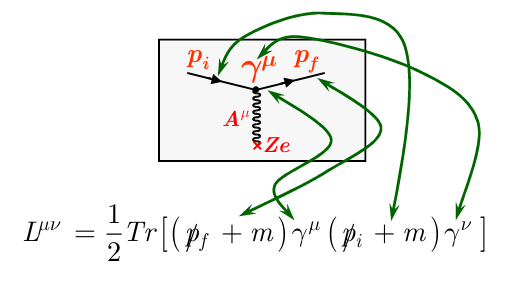
\includegraphics[width=0.7\textwidth]{Lezioni/Lezione 5/ff.png}
    \label{fig:ff}
\end{figure}
Vedremo che i calcoli che abbiamo fatto possono esssere messi in relazione a diagrammi: I Diagrammi di Feynman. Ad esempio il calcolo perturbativo al primo ordine dello scattering di Coulomb per un fermione ha come diagramma: una corrente elettromagnetica
$$
j^\mu = -ie\overline{u}(p_f, s_f)\gamma^\mu u(p_i, s_i)
$$
Interagisce con un fotone vituale (potenziale) $A_\mu$ emesso da un nucleo. A questo diagramma si può associare automaticamente il tensore leptonico
$$
L^{\mu\nu} = \frac{1}{2}Tr[(\slashed{p}_f + m)\gamma^\mu (\slashed{p}_i + m)\gamma^\nu]
$$
Questa espressione si scrive percorrendo da destra a sinistra il diagramma
\begin{itemize}
    \item Stato finale: $\slashed{p}_f + m$
    \item Vertice: $\gamma^\mu$
    \item Stato iniziale: $\slashed{p}_i + m$
    \item Vertice $\gamma^\nu$
\end{itemize}
\section{Effetti di polarizzazione}
In alcuni casi il metodo delle tracce introdotto non è direttamente utilizzabile. Infatti non si può quando si utilizza un fascio polarizzato o se si vuole misurare la polarizzazionenello stato finale. Tuttavia è possibile utilizzare una strategia simile; rivediamo i punti essenziali del metodo introdotto:
\begin{itemize}
    \item Per limitare la somma agli stati di energia positiva abbiamo utilizzato i proiettori di energia positiva e negativa $\Lambda_{\pm}$
    \item In tal modo si può estendere la somma agli stati di energia negativa
    \item I proiettori ci assicurano che questi (stati $p_0<0$) non contribuiscono effettivamente alla somma
    \item La linearità dei proiettori permette di fare prima la somma su tutti gli stati e solo successivamente applicare il proiettore.
\end{itemize}
Un metodo analogo per studiare la polarizzazione richiede i proiettori di spin. Vogliamo costruire un operatore con le seguenti proprietà
$$
P_\Sigma(s) u(\mathbf{p}, s) = u(\mathbf{p}, s) \qquad P_\Sigma(s) v(\mathbf{p}, s) = v(\mathbf{p}, s)
$$
$$
P_\Sigma(-s) u(\mathbf{p}, s) = 0 \qquad P_\Sigma(-s) v(\mathbf{p}, s) = 0
$$
Alcune importanti proprietà di questi operatori:
$$
P_\Sigma(s) + P_\Sigma(-s) = I \qquad P_\Sigma(s) P_\Sigma(-s) = 0
$$
$$
P_\Sigma(s) P_\Sigma(s) = P_\Sigma(s)
$$
$$
P_\Sigma(-s) P_\Sigma(-s) = P_\Sigma(-s)
$$
Nel calcolo del tensore leptonico $L^{\mu\nu}$ siamo partiti dall'espressione
$$
L^{\mu\nu} = \frac{1}{2} \sum_{\sigma_1=\pm s_f, \sigma_2=\pm s_i} (\overline{u}(p_f, \sigma_1)\gamma^\mu u(p_i, \sigma_2))(\overline{u}(p_i, \sigma_2)\gamma^\nu u(p_f, \sigma_1))
$$
Supponiamo che lo stato iniziale sia polarizzato: non abbiamo più la somma sugli stati iniziali (somma su $\sigma_2$)
$$
L^{\mu\nu} = \cancel{\frac{1}{2}}\sum_{\sigma_1=\pm s_f} (\overline{u}(p_f, \sigma_1)\gamma^\mu u(p_i, \sigma_2))(\overline{u}(p_i, \sigma_2)\gamma^\nu u(p_f, \sigma_1))
$$
Inoltre, dal momento che rimane un solo stato, si elimina la media. Per poter utilizzare le relazioni di completezza occorre reintrodurre la somma sulla polarizzazione iniziale! Possiamo utilizzare i proiettori di spin
$$
P_\Sigma(s_i) u(p_i, s_i) = u(p_i, s_i) \qquad P_\Sigma(s_i) u(p_i, -s_i) = 0
$$
Se introduciamo il proiettore possiamo estendere di nuovo la somma ai due stati di polarizzazione
$$
L^{\mu\nu} = \sum_{\sigma_1=\pm s_f, \textcolor{red}{\sigma_2=\pm s_i}} (\overline{u}(p_f, \sigma_1)\gamma^\mu \textcolor{red}{P_\Sigma(s_i)} u(p_i, \sigma_2))(\overline{u}(p_i, \sigma_2)\gamma^\nu u(p_f, \sigma_1))
$$
Da notare che è sufficiente introdurre $P_\Sigma$ una sola volta! Da questo punto in poi il calcolo procede come nel caso senza polarizzazione. Si arriva al risultato
$$
L^{\mu\nu} = Tr[(\slashed{p}_f + m)\gamma^\mu \textcolor{red}{P_\Sigma(s_i)}(\slashed{p}_i + m)\gamma^\nu]
$$
Analogamente, se si volesse misurare la polarizzazione dello stato finale si introdurrebbe il proiettore $P_\Sigma(s_f)$
$$
L^{\mu\nu} = Tr[\textcolor{red}{P_\Sigma(s_f)}(\slashed{p}_f + m)\gamma^\mu (\slashed{p}_i + m)\gamma^\nu]
$$
pertanto abbiamo bisogno degli operatori di proiezioni che antipiamo avere la forma:
$$
P_\Sigma(\pm s) = \frac{1 \pm \gamma_5 \slashed{s}}{2}
$$
Il tensore leptonico, per una polarizzazione $+s_i$ dello stato iniziale diventa
$$
L^{\mu\nu} = Tr\left[(\slashed{p}_f + m)\gamma^\mu \frac{1 + \gamma_5 \slashed{s}_i}{2} (\slashed{p}_i + m)\gamma^\nu\right]
$$
\section{Proiettori di Spin}
Il problema è che abbiamo visto che quando la particella è in movimento lo spin non si conserva. Questo è dovuto al fatto che nella Hamiltoniana della particella libera dell'equazione di Dirac compare il termine $\boldsymbol{\alpha}\cdot\boldsymbol{p}$ gli $\boldsymbol{\alpha}$ sono legati ai generatori delle rotazioni e quindi allo spin della particella e questo accoppiamento tra quantità di moto e spin fa in modo che lo spin non si conserva. Nel sistema di riposo questo termine non c'è in quanto $\boldsymbol{p}$ è nullo e quindi in questo sistema lo spin si conserva. Quando parliamo di polarizzazione di una particella intendiamo: vado nel sistema di riposo di una particella vedo quale è la sua polarizzazione e definisco quella polarizzazione della particella sia nello stato finale che iniziale però devo fare questo passaggio dal sistema dove è in movimento fino al rest frame.
Approfondiamo innanzitutto il significato dei proiettori di spin. Lo spin non si conserva per una particella in movimento. Abbiamo introdotto lo spin facendo riferimento al sistema di riposo. Nel sistema di riposo la definizione di un proiettore è semplice. Io voglio qualcosa che nel sistema di riposo della particella proietti una polarizzazione rispetto ad un'altra. L'operatore di spin è $S=\frac{1}{2}\Sigma$ dove $\Sigma$ lo abbiamo rappresentato grazie ai generatori delle trasformazioni di Lorentz con indici $k,l$ (escluso indice $0$)
$$
\boldsymbol{\Sigma}^j = \sigma^{kl} = i\gamma^k\gamma^l
$$
E non dipende dalla rappresentazione. I possibili stati di un fermione non possono essere descritti con i due spinori $u$ con $p=0$ e con polarizzazione $\pm\boldsymbol{\xi}$
$$
u(0, \pm s') \qquad s'^\nu=(0,\pm\boldsymbol{\xi})
$$
Come nella teoria non relativistica si ha
$$
(\boldsymbol{\Sigma} \cdot \boldsymbol{\xi}) u(0, \pm s') = \pm u(0, \pm s')
$$
Quindi questi spinori che sto utilizzando caratterizzati dalla polarizzazione sono autovalori di questo operatore.
E anche questo non dipende dalla rappresentazione. Pertanto, nel sistema di riposo, i proiettori sono semplicemente
$$
P_\Sigma(+\boldsymbol{\xi}) = \frac{1 + \boldsymbol{\Sigma} \cdot \boldsymbol{\xi}}{2} \qquad P_\Sigma(-\boldsymbol{\xi}) = \frac{1 - \boldsymbol{\Sigma} \cdot \boldsymbol{\xi}}{2}
$$
si ha ovviamente
$$
P_\Sigma(+\boldsymbol{\xi}) u(0, s') = u(0, s') \qquad P_\Sigma(+\boldsymbol{\xi}) u(0, -s') = 0
$$
$$
P_\Sigma(-\boldsymbol{\xi}) u(0, s') = 0 \qquad P_\Sigma(-\boldsymbol{\xi}) u(0, -s') = u(0, -s')
$$
Estendiamo le definizioni alle soluzioni di energia negativa $v$. Abbiamo una complicazione (in un ipotetico esperimento di Stern-Gerlach non interessa all'apparato se ho una particella o antiparticella ma solo dallo spin verso l'alto o verso il basso. Il problema è che la rappresentazione matematica dello spin nell'equazione di Dirac è invertita) aggiuntiva infatti l'interpretazione di hole associa lo spin fisico agli autovalori di $\Sigma\cdot\xi$ con i segni invertiti
\begin{figure}[h!]
    \centering
    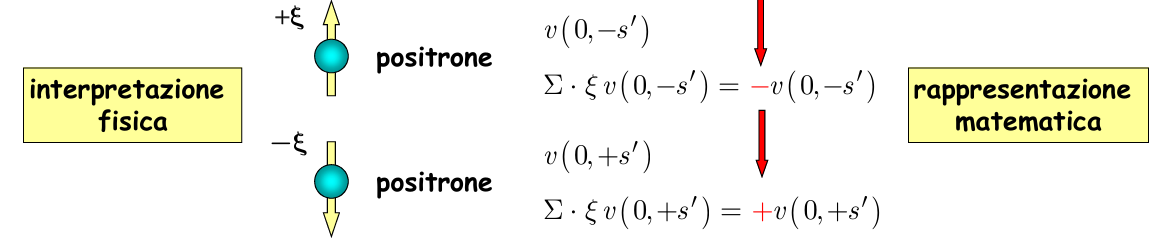
\includegraphics[width=0.8\textwidth]{Lezioni/Lezione 5/sa.png}
    \label{fig:sa}
\end{figure}
Il valore della grandezza fisica associata all'antiparticella è l'autovalore in rosso cambiato di segno. Ovviamente vogliamo un formalismo che superi questa difficoltà. Un operatore il cui autovalore abbia il segno corretto automaticamente. Possiamo utilizzare la proprietà che gli spinori $u$ e $v$ sono autovettori di $\gamma^0$ con autovalori $\pm1$ rispettivamente
$$
\gamma^0u(0,s)=+u(0,s) \qquad \gamma^0v(0,s)=-v(0,s)
$$
Possiamo modificare l'operatore $\xi\cdot\Sigma$ nel seguente modo
$$
\boldsymbol{\xi}\cdot\boldsymbol{\Sigma} \quad \Longrightarrow \quad \boldsymbol{\xi}\cdot\boldsymbol{\Sigma}\gamma^0
$$
Con questo operatore ovviamente
\begin{figure}[h!]
    \centering
    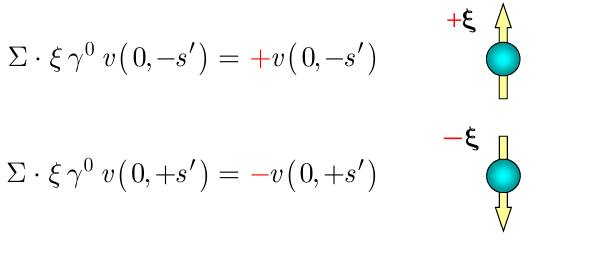
\includegraphics[width=0.8\textwidth]{Lezioni/Lezione 5/fa.png}
    \label{fig:fa}
\end{figure}
Per quanto riguarda gli spinori $u$ non cambia nulla dato che $\gamma^0u=u$. Gli operatori di proiezione, nel sistema di riposo, sono pertanto:
$$
P_\Sigma(+\boldsymbol{\xi}) = \frac{1 + \boldsymbol{\xi} \cdot \boldsymbol{\Sigma}\gamma^0}{2} \qquad P_\Sigma(-\boldsymbol{\xi}) = \frac{1 - \boldsymbol{\xi} \cdot \boldsymbol{\Sigma}\gamma^0}{2}
$$
Proiettano gli stati con polarizzazione FISICA $\pm\boldsymbol{\xi}$ e si comportano allo stesso modo per gli spinori $u$ e $v$. Fin qui abbiamo fatto considerazioni nel sistema di riposo della particella. Possiamo ottenere gli spinori per una particella in movimento con una trasformazione di Lorentz
\begin{figure}[h!]
    \centering
    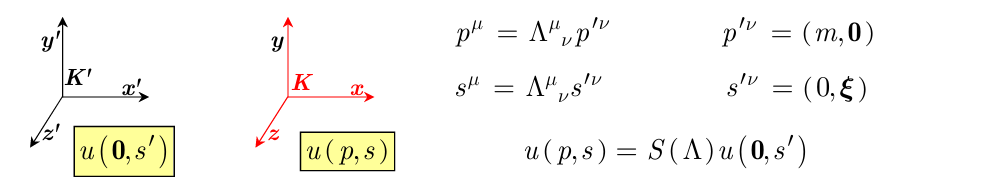
\includegraphics[width=0.8\textwidth]{Lezioni/Lezione 5/la.png}
    \label{fig:la}
\end{figure}
Vogliamo trovare un operatore che svolta il ruolo di $\boldsymbol{\xi} \cdot \boldsymbol{\Sigma}\gamma^0$ nel sistema $\mathbf{K}$, che agisca direttamente sugli spinori $u(p,s)$ e $v(p,s)$ e che abbia autovalori $+1$ e $-1$ uguali a quelli di $\boldsymbol{\xi} \cdot \boldsymbol{\Sigma}\gamma^0$ nel sistema di riposo. Cominciamo con scrivere in modo covariante l'operatore $\boldsymbol{\xi} \cdot \boldsymbol{\Sigma}\gamma^0$ nel sistema $\mathbf{K}'$
$$
\Sigma^j=\sigma^{kl}=i\gamma^k\gamma^l \qquad \Sigma^j=-i\gamma^1\gamma^2\gamma^3\gamma^j
$$
Utilizzando l'ultima espressione (e sotto intesa la somma su $j=1,2,3$)
$$
\boldsymbol{\Sigma} \cdot \boldsymbol{\xi} \gamma^0 = \xi^j \Sigma^j \gamma^0 = -i \xi^j \gamma^1 \gamma^2 \gamma^3 \gamma^j \gamma^0 = -i \xi^j \gamma^0 \gamma^1 \gamma^2 \gamma^3 \gamma^j = - \xi^j \gamma^5 \gamma^j
$$
Riepilogando $(j=1,2,3)$
$$
\boldsymbol{\Sigma} \cdot \boldsymbol{\xi} \gamma^0=- \xi^j \gamma^5 \gamma^j
$$
Dal momento che nel sistema di riposo $s'^\nu=(0,\xi)$ possiamo scrivere
$$
\boldsymbol{\xi} \cdot \boldsymbol{\Sigma}\gamma^0 = -\xi^j \gamma^5 \gamma^j = \gamma^5 s_\nu \gamma^\nu = \gamma^5 \slashed{s}
$$
Si può dimostrare che l'operatore $\gamma^5 \slashed{s}'$ si trasforma nell'operatore $\gamma^5 \slashed{s}$. Vale a dire: l'operatore $\gamma^5\slashed{s}$ applicato agli spinori $u$ e $v$ nel sistema $\mathbf{K}$ dà lo stesso risultato che $\gamma^5 \slashed{s}'$ dà nel sistema di riposo $\mathbf{K}'$
$$
\gamma^5 \slashed{s} u(p, \pm s) = \pm u(p, \pm s) \qquad \gamma^5 \slashed{s} v(p, \pm s) = \pm v(p, \pm s)
$$
Abbiamo pertanto trovato l'operatore che applicato agli spinori di particelle in moto ci dice quale è lo spin nel sistema di riposo. Ovviamente gli operatori
$$
P_\Sigma(\pm s) = \frac{1 \pm \gamma_5 \slashed{s}}{2}
$$
sono gli operatori di proiezione che cercavamo.
\section{Proiezione nella diffusione di Coulomb}
Studiamo adesso eventuali effetti dovuti alla polarizzazione nella diffusione di Coulomb. Vedremo che la sezione d'urto non dipende dalla polarizzazione iniziale ma ricordiamo che tuttavia le formule sono approssimate al primo ordine. Vedremo che la sezione d'urto dipende dalla polarizzazione iniziale solo al secondo ordine. Utilizzeremo questo effetto per studiare la polarizzazione dell'elettrone nel decadimento beta. Calcoliamo la sezione d'urto per un elettrone con polarizzazione iniziale $s_i$. Abbiamo visto che in questo caso il tensore $L^{\mu\nu}$ diventa
$$
L^{\mu\nu} = Tr\left[(\slashed{p}_f + m)\gamma^\mu \textcolor{red}{\frac{1 + \gamma_5 \slashed{s}_i}{2}} (\slashed{p}_i + m)\gamma^\nu\right]
$$
Sviluppando si ottiene
$$
L^{\mu\nu} = Tr\left[(\slashed{p}_f + m)\gamma^\mu \textcolor{red}{\frac{1}{2}} (\slashed{p}_i + m)\gamma^\nu\right] + Tr\left[(\slashed{p}_f + m)\gamma^\mu \textcolor{red}{\frac{\gamma_5 \slashed{s}_i}{2}} (\slashed{p}_i + m)\gamma^\nu\right]
$$
Il primo termine è identico a quello del caso senza polarizzazione, sviluppando il secondo termine diventa
$$
\frac{1}{2} Tr[\slashed{p}_f \gamma^\mu \gamma_5 \slashed{s}_i \slashed{p}_i \gamma^\nu + m\slashed{p}_f \gamma^\mu \gamma_5 \slashed{s}_i \gamma^\nu + m\gamma^\mu \gamma_5 \slashed{s}_i \slashed{p}_i \gamma^\nu + m^2\gamma^\mu \gamma_5 \slashed{s}_i \gamma^\nu]
$$
Analizziamo i vari termini: il primo e l'ultimo sono nulli in quanto ho un numero dispari di matrici $\gamma$ ($\gamma^5$ equivale a 4 matrici $\gamma$). Il secondo e il terzo sono diversi da zero. Ad esempio 
$$
Tr[\gamma^5 \gamma^\mu \gamma^\nu \gamma^\rho \gamma^\sigma] = 4i \varepsilon^{\mu\nu\rho\sigma}
$$
$$
Tr[\slashed{p}_f \gamma^\mu \gamma_5 \slashed{s}_i \gamma^\nu] = p_{f\rho} s_{i\sigma} Tr[\gamma_5 \gamma^\rho \gamma^\mu \gamma^\sigma \gamma^\nu] = 4i p_{f\rho} s_{i\sigma} \varepsilon^{\rho\mu\sigma\nu}
$$
Tuttavia, nella diffusione Coulombiana il campo elettrostatico fa sopravvivere solo il termine $\mu=\nu=0$ e pertanto il termine è nullo (antisimmetria di $\varepsilon^{\rho\mu\sigma\nu}$). Concludiamo che, al primo ordine, la sezione d'urto non dipende dalla polarizzazione iniziale.
\section{Tracce con la matrice gamma 5}
Riportiamo alcune tracce che coinvolgono la matrice $\gamma^5=i\gamma^0\gamma^1\gamma^2\gamma^3$. Innanzitutto 
$$
Tr[\gamma^5] = 0
$$
Infatti $\gamma^5$ contiene tutte e 4 le matrici $\gamma$. La traccia di 4 matrici $\gamma$ porta ad una espressione che contiene tre tensori $g^{\mu\nu}$ con indici tutti differenti e quindi il risultato è zero. Inoltre
$$
Tr[\gamma^5\gamma^\mu\gamma^\nu] = 0
$$
\begin{itemize}
    \item se $\mu=\nu$ rimane la traccia di $\gamma^5$ e quindi il risultato è zero
    \item Se $\mu\not=\nu$ allora con opportune commutazioni le due matrici $\gamma$ possono essere portate in posizioni adiacenti alle corrispondenti matrici in $\gamma^5$. Il prodotto è $\pm1$ e si eliminano quindi 2 matrici $\gamma$. Rimane la traccia di 2 matrici con indici differenti quindi nulla.
\end{itemize}
Per finire
$$
Tr[\gamma^5\gamma^\mu\gamma^\nu\gamma^\rho\gamma^\sigma] = 4i\varepsilon^{\mu\nu\rho\sigma}
$$
$$
\varepsilon_{0123} = -\varepsilon^{0123} = 1
$$
Innanzitutto i 4 indici devono essere tutti differenti altrimenti, con opportune commutazioni si torna ai casi precedenti
$$
4 = Tr[I] = Tr[\gamma^5\gamma^5] = Tr[\gamma^5 i\gamma^0\gamma^1\gamma^2\gamma^3] \qquad Tr[\gamma^5\gamma^0\gamma^1\gamma^2\gamma^3] = -4i = 4i\varepsilon^{0123}
$$
\section{Polarizzazione nella diffusione di Coulomb}
Generalizzando le regole per scrivere l'elemento di matrice direttamente dal diagramma di Feynman al caso in cui i fermioni iniziale e finale siano polarizzati. Si percorre da destra a sinistra il diagramma:
\begin{itemize}
    \item Stato finale con polarizzazione $s_f$
$$
\textcolor{red}{\frac{1 + \gamma_5 \slashed{s}_f}{2}} (\slashed{p}_f + m)
$$
\item Vertice (interazione vettoriale) $\gamma^\mu$
    \item Stato iniziale con polarizzazione $s_i$
$$
\textcolor{red}{\frac{1 + \gamma_5 \slashed{s}_i}{2}} (\slashed{p}_i + m)
$$
\item Vertice $\gamma^\nu$
\end{itemize}
\begin{figure}[h!]
    \centering
    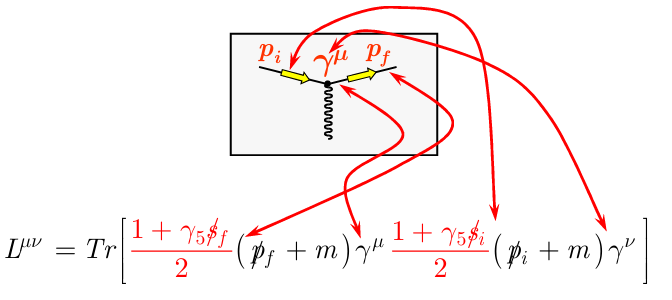
\includegraphics[width=0.8\textwidth]{Lezioni/Lezione 5/yy.png}
    \label{fig:yy}
\end{figure}
Calcoliamo adesso la polarizzazione dello stato finale per una data polarizzazione dello stato iniziale. In generale la polarizzazione è data da
$$
P=\frac{N_+-N_-}{N_++N_-}
$$
Le quantità $N_+$ e $N_-$ sono il numero di particelle con polarizzazione rispettivamente parallela o antiparallela all'asse di quantizzazione. Il numero di interazioni è proporzionale al modulo quadrato dell'elemento di matrice
\begin{figure}[h!]
    \centering
    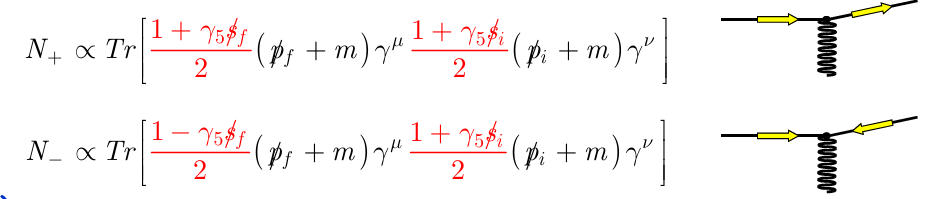
\includegraphics[width=0.9\textwidth]{Lezioni/Lezione 5/ly.png}
    \label{fig:ly}
\end{figure}
è evidente che nella somma $N_++N_-$ la dipendenza da $s_f$ si cancella. Nel denominatore rimane solo la dipendenza da $s_i$. Abbiamo visto nello scattering Coulombiano che $\gamma_5\slashed{s}$ non contribuisce. IL risultato è
$$
N_+ + N_- \propto L^{00} = 4\left[E^2 - \mathbf{p}^2 \sin^2 \frac{\theta}{2}\right] = 4\left[E^2 \cos^2 \frac{\theta}{2} + m^2 \sin^2 \frac{\theta}{2}\right]
$$
$$
N_+ \propto Tr\left[\frac{1 + \gamma_5 \slashed{s}_f}{2} (\slashed{p}_f + m) \gamma^\mu \frac{1 + \gamma_5 \slashed{s}_i}{2} (\slashed{p}_i + m) \gamma^\nu\right]
$$
$$
N_- \propto Tr\left[\frac{1 - \gamma_5 \slashed{s}_f}{2} (\slashed{p}_f + m) \gamma^\mu \frac{1 + \gamma_5 \slashed{s}_i}{2} (\slashed{p}_i + m) \gamma^\nu\right]
$$
Valutiamo adesso il numeratore. Notiamo che i termini $1\pm\gamma_5\slashed{s}_f$ danno origine alle espressioni
$$
\frac{1}{2}(\slashed{p}_f + m)\gamma^\mu \frac{1 + \gamma_5 \slashed{s}_i}{2} (\slashed{p}_i + m)\gamma^\nu \qquad \pm \frac{\gamma_5 \slashed{s}_f}{2} (\slashed{p}_f + m)\gamma^\mu \frac{1 + \gamma_5 \slashed{s}_i}{2} (\slashed{p}_i + m)\gamma^\nu
$$
Nell'espressione $N_+-N_-$ la prima espressione si elide pertanto sopravvive solo
$$
N_+ - N_- \propto Tr\left[\gamma_5 \slashed{s}_f (\slashed{p}_f + m)\gamma^\mu \frac{1 + \gamma_5 \slashed{s}_i}{2} (\slashed{p}_i + m)\gamma^\nu\right]
$$
Sviluppando l'espressione
$$
N_+ - N_- \propto \frac{1}{2}Tr[(\gamma_5 \slashed{s}_f \slashed{p}_f \gamma^\mu + \gamma_5 \slashed{s}_f m \gamma^\mu)(1 + \gamma_5 \slashed{s}_i)(\slashed{p}_i \gamma^\nu + m\gamma^\nu)]
$$
$$
N_+ - N_- \propto \frac{1}{2}Tr\left[
\begin{aligned}
&\gamma_5 \slashed{s}_f \slashed{p}_f \gamma^\mu \slashed{p}_i \gamma^\nu + \gamma_5 \slashed{s}_f \slashed{p}_f \gamma^\mu m \gamma^\nu + \gamma_5 \slashed{s}_f \slashed{p}_f \gamma^\mu \gamma_5 \slashed{s}_i \slashed{p}_i \gamma^\nu + \gamma_5 \slashed{s}_f \slashed{p}_f \gamma^\mu \gamma_5 \slashed{s}_i m \gamma^\nu + \\
&\gamma_5 \slashed{s}_f m \gamma^\mu \slashed{p}_i \gamma^\nu + \gamma_5 \slashed{s}_f m \gamma^\mu m \gamma^\nu + \gamma_5 \slashed{s}_f m \gamma^\mu \gamma_5 \slashed{s}_i \slashed{p}_i \gamma^\nu + \gamma_5 \slashed{s}_f m \gamma^\mu \gamma_5 \slashed{s}_i m \gamma^\nu
\end{aligned}
\right]
$$
L'espressione trovata è più semplice di quanto appaia a prima vista. Analizziamo i vari termini nell'ordine:
\begin{enumerate}
    \item Nullo: numero dispari di matrici $\gamma$
    \item Non contribuisce: la traccia è proporzionale a $\varepsilon^{\rho\sigma\mu\nu}$ che è $0$ per $\mu=\nu$
    \item Da calcolare
    \item Nullo: numero dispari di matrici $\gamma$
    \item Come il punto 2)
    \item Nullo: numero dispari di matrici $\gamma$
    \item Nullo: numero dispari di matrici $\gamma$
    \item Da calcolare
\end{enumerate}
Pertanto sopravvivono solo due termini
$$
N_+ - N_- \propto \frac{1}{2}Tr\left[ \gamma_5 \slashed{s}_f \slashed{p}_f \gamma^\mu \gamma_5 \slashed{s}_i \slashed{p}_i \gamma^\nu + \gamma_5 \slashed{s}_f m \gamma^\mu \gamma_5 \slashed{s}_i m \gamma^\nu \right]
$$
Le matrici $\gamma^5$ possono essere eliminate con opportune commutazioni
$$
N_+ - N_- \propto \frac{1}{2}Tr[+m^2 \slashed{s}_f \gamma^\mu \slashed{s}_i \gamma^\nu - \slashed{s}_f \slashed{p}_f \gamma^\mu \slashed{p}_i \gamma^\nu]
$$
Il primo termine è del tipo già visto
$$
Tr[\gamma^\rho \gamma^\mu \gamma^\sigma \gamma^\nu] = 4(g^{\rho\mu}g^{\sigma\nu} + g^{\rho\nu}g^{\mu\sigma} - g^{\rho\sigma}g^{\mu\nu})
$$
\begin{align*}
s_{f\rho} s_{i\sigma} Tr[\gamma^\rho \gamma^\mu \gamma^\sigma \gamma^\nu] &= 4s_{f\rho} s_{i\sigma} (g^{\rho\mu}g^{\sigma\nu} + g^{\rho\nu}g^{\mu\sigma} - g^{\rho\sigma}g^{\mu\nu}) \\
&= 4(s_f^\mu s_i^\nu + s_f^\nu s_i^\mu - s_f \cdot s_i g^{\mu\nu})
\end{align*}
Per il secondo termine occorre una nuova regola
\begin{align*}
Tr[\gamma^{\mu_1} \gamma^{\mu_2} \gamma^{\mu_3} \dots \gamma^{\mu_n}] &=
\end{align*}
$$
= g^{\mu_1\mu_2}Tr[\gamma^{\mu_3} \dots \gamma^{\mu_n}] - g^{\mu_1\mu_3}Tr[\gamma^{\mu_2} \dots \gamma^{\mu_n}] + \dots + g^{\mu_1\mu_n}Tr[\gamma^{\mu_2} \dots \gamma^{\mu_{n-1}}]
$$
Lo sviluppo dell'espressione è lasciata com e esercizio, per il risultato finale occorre inoltre definire i vettori di spin $s_i$ e $s_f$. Definiamo i vettori di polarizzazione utilizzando le proiezioni lungo $p_i$ e $p_f$. Ricordiamo la definizione del vettore $s$.
$$
s^0 = \frac{|\mathbf{p}|}{m} \boldsymbol{\xi}_{||} \qquad s_\perp = \boldsymbol{\xi}_\perp \qquad s_{||} = \frac{E}{m} \boldsymbol{\xi}_{||}
$$
Per la particella nello stato iniziale quantizziamo lo spin nella direzione del momento incidente
\begin{figure}[h!]
    \centering
    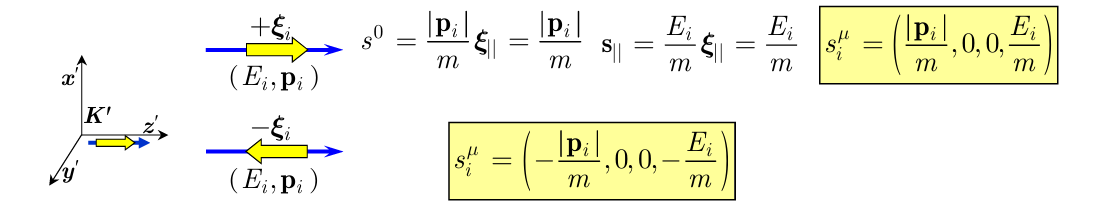
\includegraphics[width=0.8\textwidth]{Lezioni/Lezione 5/po.png}
    \label{fig:po}
\end{figure}
Per la particella nello stato finale quantizziamo lo spin nella direzione del momento uscente
\begin{figure}[h!]
    \centering
    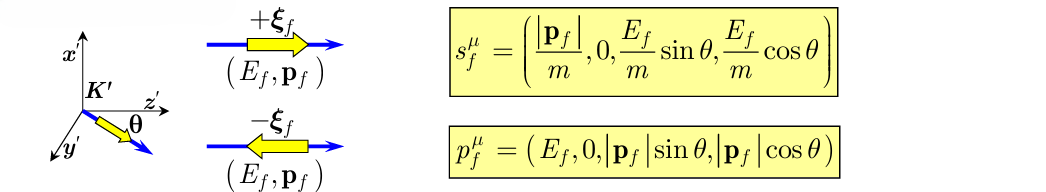
\includegraphics[width=0.8\textwidth]{Lezioni/Lezione 5/pi.png}
    \label{fig:pi}
\end{figure}
Utilizzando le formule ricavate e i vettori polarizzazione $s$ il risultato è

L'interpretazione di questo risultato è la seguente: lo stato iniziale è completamente polarizzato (dato del problema) e abbiamo scelto polarizzazione lungo $p$ (elicità Right-Handed). Lo stato finale ha una polarizzazione che dipende dall'angolo. La probabilità relativa di uno stato finale Right-Handed o di uno stato Left-Handed dipende dall'angolo. Alucni casi notevoli:
\begin{itemize}
    \item $\theta=0\to P=1$
    \item $\theta=\pi\to P=-1$
    \item $\beta\ll1$ $(E\to m)$ $P=1-2\sin^2{\frac{\theta}{2}}=\cos{\theta}$ questo vuol dire che la probabilità che la particella abbia uno spin che fa un angolo $\theta$ è $\cos(\theta)$. Questo significa che lo spin rimane nella stessa direzione e cioè che lo spin si conserva. Perché quando la particella è polarizzata ma non nella direzione in cui vado ad osservarla io misuro la proiezione lungo quella direzione. Nel limite non relativistico io noto la conservazione dello spin non deve essere una sorpresa. Abbiamo già visto che a limite non relativistico lo spin non si accoppia con il campo elettrico.
    \item $\beta\to 1$ $(E\gg m)$ $P=1$ nel limite ultrarelativistico si conserva l'elicità.
\end{itemize}
\section{Conservazione dell'elicità}
Quando la particella è ultra-relativistica il $4-$vettore di spin assume una forma limite interessante. Consideriamo lo spin nella direzione del momento $\boldsymbol{\xi}_{||}=1$ $\boldsymbol{\xi}_{\perp}=0$
$$
s^0 = \frac{|\mathbf{p}|}{m} \boldsymbol{\xi}_{||} \qquad s_{||} = \frac{E}{m} \boldsymbol{\xi}_{||} \qquad p^\mu=(E,0,0,|\mathbf{p}|) \quad \Rightarrow \quad s^\mu=\frac{1}{m}(|\mathbf{p}|,0,0,E)
$$
Dal momento che 
$$
|p|\to E \qquad \Longrightarrow \qquad s^\mu\to\frac{1}{m}p^\mu
$$
Ricordiamo l'espressione dei proiettori di spin
$$
P_\Sigma(\pm s) = \frac{1 \pm \gamma_5 \slashed{s}}{2}
$$
Pertanto nel caso ultra-relativistico
$$
\gamma_5 \slashed{s} u(p,s) \to \gamma_5 \frac{\slashed{p}}{m} u(p,s) \qquad (\slashed{p} - m)u = 0
$$
$$
\gamma_5 \slashed{s} u(p,s) \to \gamma_5 u(p,s)
$$
Nel caso ultrarelativistico proiezione di spin e proiezione chirale coincidono
$$
P_\Sigma(\pm s) \to \frac{1 \pm \gamma_5}{2}
$$
Pertanto nel caso ultrarelativistico gli operatori di proiezione acquistano la forma indicata che contiene solo $\gamma^5$. Inoltre dato uno spinore con polarizzazione arbitraria $u$ possiamo scomporlo nei due stati di polarizzazione usando $(1\pm\gamma^5)/2$:
\begin{itemize}
    \item Polarizzazione Right-Handed 
    $$
u_+ \approx \frac{1 + \gamma_5}{2} u
$$
    \item Polarizzazione Left-Handed
    $$
u_- \approx \frac{1 - \gamma_5}{2} u
$$
\end{itemize}
Ovviamente
$$
u_+ + u_- = u
$$
Calcoliamo anche gli aggiunti spinoriali delle due componenti. Preliminarmente osserviamo che
$$
\overline{\gamma_5} = \gamma^0 \gamma_5^\dagger \gamma^0 = \gamma^0 \gamma_5 \gamma^0 = -\gamma^0 \gamma^0 \gamma_5 = -\gamma_5
$$
$$
\overline{\gamma_5} = -\gamma_5
$$
Veniamo agli aggiunti spinoriale delle proiezioni
$$
\overline{u}_+ = \overline{\left( \frac{1 + \gamma_5}{2} u \right)} = \overline{u} \frac{1 + \overline{\gamma_5}}{2} = \overline{u} \frac{1 - \gamma_5}{2}
$$
Analogamente per $u_-$
$$
\overline{u}_+ = \overline{u} \frac{1 - \gamma_5}{2} \qquad \overline{u}_- = \overline{u} \frac{1 + \gamma_5}{2}
$$
Siamo adesso in grado di verificare che nel caso ultra-relativistico nel caso di una corrente vettoriale l'elicità è conservata. L'ampiezza per la transizione $-\to +$ è proporzionale all'elemento di matrice:
$$
\overline{u}_+ \gamma^\mu u_- = \overline{u} \frac{1}{2}(1 - \gamma_5) \gamma^\mu \frac{1}{2}(1 - \gamma_5) u = \frac{1}{4} \overline{u} [1 - (\gamma_5)^2] \gamma^\mu u
$$
$$
\overline{u}_+ \gamma^\mu u_- = 0
$$
Analogamente 
$$
\overline{u}_- \gamma^\mu u_+ = 0
$$
Sono invece diversi da zero gli elementi di matrice fra stati con la stessa elicità
\begin{align*}
\overline{u}_+ \gamma^\mu u_+ &= \overline{u} \frac{1}{2}(1 - \gamma_5) \gamma^\mu \frac{1}{2}(1 + \gamma_5) u = \frac{1}{4} \overline{u} (1 - \gamma_5) \gamma^\mu (1 + \gamma_5) u \\
&= \frac{1}{4} \overline{u} [1 + 2\gamma_5 + (\gamma_5)^2] \gamma^\mu u = \frac{1}{2} \overline{u} [1 + \gamma_5] \gamma^\mu u \neq 0
\end{align*}
